\section{Definition des Szenarioumfelds}
\label{environment}

Gegenstand des folgenden Kapitels soll es sein, relevante Umweltfaktoren herauszuheben. Dies geschieht  im Branchen- sowie im Technologiekontext des Untersuchungsobjekt Cloud Computing. 

\todo[inline]{Unternehmensumfeld (Bildungsbranche, grundsätzlich global
	Schulbuchverlage, Definition Cornelsen
	Wandel zum digitalen Lernen: Angebot der Bücher und Arbeitsmaterialien webbasiert=
	Technisches Umfeld Cloud Computing (
	Definition etc.
	Abgrenzung Private-, Public-, Community- und Hybrid-Cloud
	Abgrenzung SaaS, IaaS, PaaS)
	}

\begin{figure}
	\centering
	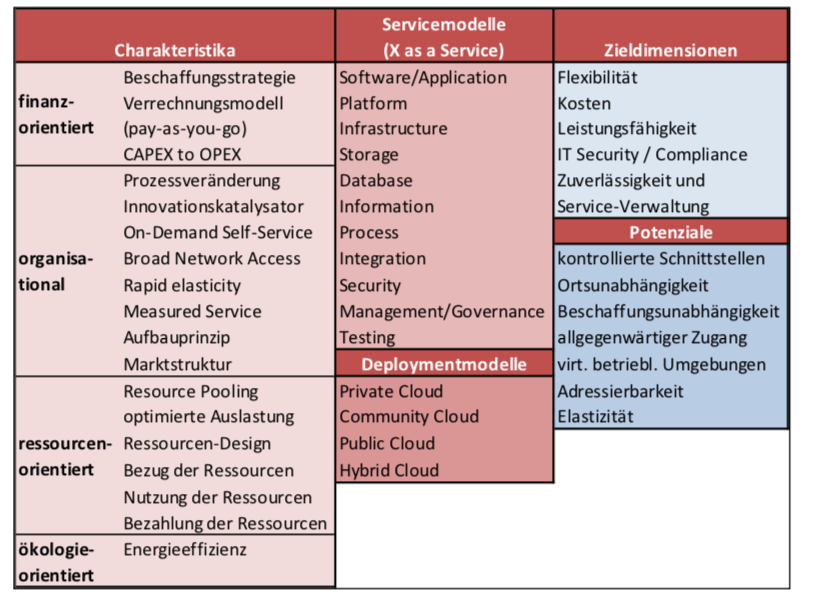
\includegraphics[width=\linewidth]{images/bigpicture}
	\caption[Caption for parameters]{ "Big Picture" des Cloud Computing nach Stieninger \cite{stieninger}}
	\label{fig:bigpicture}
\end{figure}